The system is designed to include a web-based application for visualizing maps and paths of the agents. The application is designed to be accessible via the internet, providing a user-friendly interface for monitoring the agents' movements in real-time. The web application connects to the system's data source to retrieve live data, allowing for real-time monitoring of the agent's actions and providing a powerful tool for understanding the behavior of the system. A mockup of the visualization is presented in Figure \ref{fig:vis_mock}, which illustrates the type of information that will be presented through the web application.

\begin{figure}[H]
    \centering
    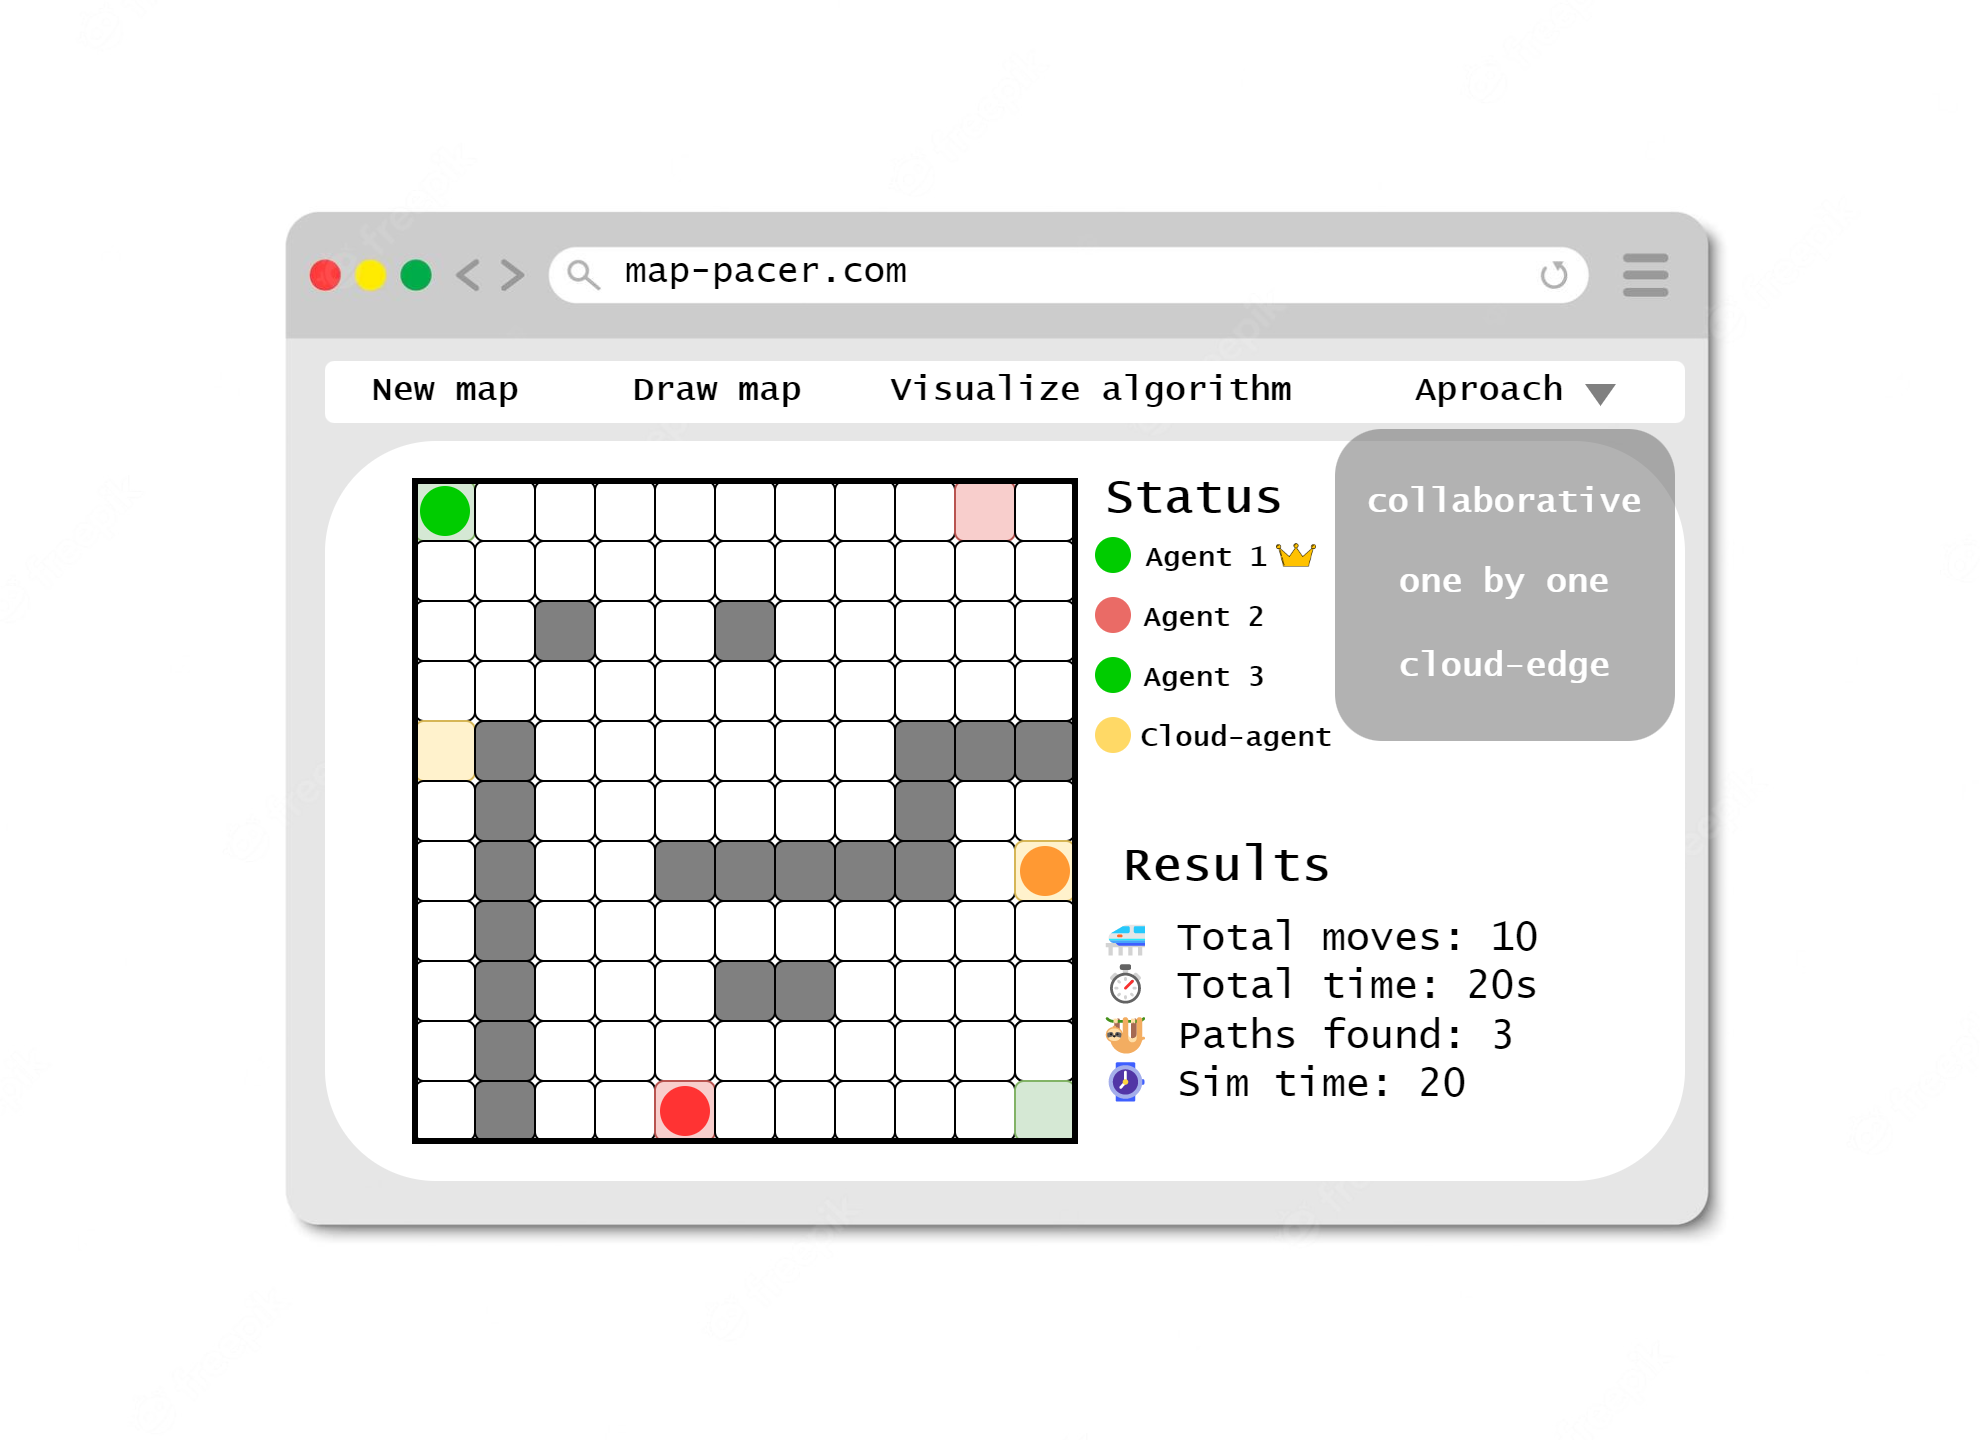
\includegraphics[width=\textwidth]{pictures/frontenf_mock.png}
    \caption{Mock of the visualization}
    \label{fig:vis_mock}
\end{figure}

The design of the graphical interface of the system is centered around a grid map, which serves to clearly display the positions and goals of all the agents as colored dots. The design also includes the display of important information such as the status of the agents, the current leader, and other relevant information pertaining to the outcome of the algorithm, all of which are presented alongside the map.

The design of the system includes a web-based application that enables the user to perform a variety of functions related to the visualization and manipulation of maps and agents. Specifically, the user will be able to:

\begin{itemize}
\itemsep0em
\item Generate new maps, either using random generation or by specifying predefined maps.
\item Create new maps by utilizing the built-in map creator feature.
\item Select from a variety of algorithms for the agents to follow.
\item Visualize the algorithm in real-time, providing a powerful tool for understanding the behavior of the system.
\end{itemize}

In addition to these core features, the system's design also incorporates a number of additional functionalities. These include the ability to:

\begin{itemize}
\itemsep0em
\item Access a map creator, allowing the user to specify their own maps.
\item Choose among different systems, providing multi-tenancy functionality.
\item Replay visualizations, allowing the user to review previous simulations.
\item Replay visualizations step-by-step, providing a detailed understanding of the behavior of the system at each stage of the algorithm.
\end{itemize}

These features are intended to provide a comprehensive and intuitive tool for understanding the behavior of the agents, and for analyzing the performance of different algorithms and maps.